\documentclass[11pt,a4paper]{article}
\usepackage{amsmath}
\usepackage{amsfonts}
\usepackage{amssymb}
\usepackage{fancyhdr}
\usepackage{lastpage}
\usepackage{graphicx}
\usepackage{ucs}
\usepackage[utf8x]{inputenc}
\usepackage[italian]{babel}

\renewcommand{\headrulewidth}{0.6pt}
\renewcommand{\footrulewidth}{0.6pt}
% impostazione dello stile per le pagine interne del documento
\lhead{\leftmark}
\chead{}
\rhead{
\includegraphics[scale=0.15]{logo.png} }
\lfoot{Piano di Progetto v0.2.0}
\cfoot{}
\rfoot{\thepage \ di \pageref{LastPage}}
% ridefinizione dello stile plain per il frontespizio
\fancypagestyle{plain}{
\fancyhf
}
% impostazione dello stile per l'indice
\fancypagestyle{indice}{
\lhead{\leftmark}
\chead{}
\rhead{
\includegraphics[scale=0.15]{logo.png}}
\lfoot{Piano di Progetto v0.2.0}
\cfoot{}
\rfoot{}
}
\headheight = 46pt
%definizione del comando "\modfiche" per la creazione del diario delle modifiche
\newcommand{\modifiche} 
{
\newpage
\begin{center}
\textbf{Diario delle modifiche} \\
\bigskip
\begin{tabular}{|c|c|p{0.69\textwidth}|}
\hline
\textsc{Data} & \textsc{Versione} & \textsc{Modifica} \\
\hline
\hline
\textit{29-11-2008} & 0.1.0 & Prima bozza del documento \\
\hline
\hline
\textit{02-12-2008} & 0.2.0 & Inserimento tabelle e Gantt \\
\hline
\end{tabular}
\end{center}
}
%definizione del comando "\info" per la creazione delle informazioni del documento
\newcommand{\info} {
\bigskip
\begin{tabbing}
	\hspace*{0.3\textwidth} \= \hspace*{0.5\textwidth} \kill
	\parbox{0.3\textwidth}{\textbf{Verifica: }} \> \parbox{0.5\textwidth}{Freo Matteo} \\
	\parbox{0.3\textwidth}{\textbf{Approvazione: }} \> \parbox{0.5\textwidth}{Grosselle Alessandro} \\
	\parbox{0.3\textwidth}{\textbf{Stato: }} \> \parbox{0.5\textwidth}{Preliminare} \\
	\parbox{0.3\textwidth}{\textbf{Uso: }} \> \parbox{0.5\textwidth}{Esterno} \\
	\parbox{0.3\textwidth}{\textbf{Distribuzione: }} \> \parbox{0.5\textwidth}{QuiXoft} \\
	\> \parbox{0.5\textwidth}{Rossi Francesca} \\
	\> \parbox{0.5\textwidth}{Vardanega Tullio} \\
\end{tabbing}
}
%definizione del comando "\frontespizio" per la creazione del frontespizio
\newcommand{\frontespizio} {
\thispagestyle{plain}
\title{\begin{Huge}\textsc{Progetto SIGEOL}\end{Huge} \\ \textit{Piano di Progetto \\ v0.2.0}}
\author{Redazione: Grosselle Alessandro}
\maketitle
\medskip
\begin{center}

\includegraphics[scale=0.5]{logo.png} \\
\textit{quixoft.sol@gmail.com}
\end{center}
\medskip
\info
\newpage
}
%definizione del comando "\indice" per la creazione dell'indice
\newcommand{\indice} {
\thispagestyle{indice}
\tableofcontents
\newpage
}
\pagestyle{fancy}
\begin{document}
\frontespizio
\indice
\setcounter{page}{1}
\section{Introduzione}
\subsection{Scopo del prodotto}
Lo scopo del prodotto ''SIGEOL'' è di fornire un sistema software per la gestione dell’orario di lezione a uso del CCS di Informatica.
\subsection{Scopo del documento}
Questo documento espone la pianificazione del progetto ''SIGEOL''.
Al suo interno è possibile trovare una stima delle tempistiche e dei costi del progetto; il tutto è illustrato attraverso l’utilizzo di tabelle e del diagramma di Gantt.
La ripartizione dei ruoli tiene conto del fatto che tutti devono avere circa lo stesso carico di lavoro.
\subsection{Glossario}
Il glossario è unico per tutti i documenti relativi al progetto di sviluppo del prodotto e viene fornito come allegato nel file Glossario.pdf.
\section{Organigramma}
\subsection{Accettazione delle componenti}

\begin{tabular}{|c|c|c|}
\hline
Nominativo  & Data & Firma(leggibile) \\ \hline
Barbiero Mattia & 12/11/08 & \multicolumn{1}{l|}{} \\ \hline
Beggiato Andrea & 12/11/08 &  \\ \hline
Freo Matteo & 12/11/08 &  \\ \hline
Grosselle Alessandro & 12/11/08 &  \\ \hline
Scarpa Davide & 12/11/08 &  \\ \hline
Scortecagna Carlo & 12/11/08 &  \\ \hline
\end{tabular}


\subsection{Descrizione delle componenti}

\begin{tabular}{|c|c|c|}
\hline
Nominativo  & Matricola & e-mail \\ \hline
Barbiero Mattia & 540546 & barraemme@gmail.com \\ \hline
Beggiato Andrea & 541738 & saprus@hotmail.it \\ \hline
Freo Matteo & 560838 & tizzy369@hotmail.it \\ \hline
Grosselle Alessandro & 540501 & ale7forever@gmail.com \\ \hline
Scarpa Davide & 544006 & goldmagic@libero.it \\ \hline
Scortecagna Carlo & 545070 & carloscortecagna@gmail.com \\ \hline
\end{tabular}

\subsection{Criteri di assegnazione}
In ogni fase, tutti i membri assumeranno due ruoli.
Il cambio del ruolo avverrà a metà di ogni fase e in quel momento ogni componente dovrà aver speso tutte le ore assegnateli per svolgere il ruolo dato.
Si ipotizzano le seguenti date:\\

\begin{tabular}{|c|c|c|}
\hline
Fase & Inizio  & Termine \\ \hline
Analisi dei requisiti & 17/11/08 & 23/12/08 \\ \hline
Progettazione & 07/01/09 & 14/02/09 \\ \hline
Codifica & 16/02/09 & 11/03/09 \\ \hline
Verifica e validazione & 17/03/09 & 24/03/09 \\ \hline
\end{tabular}
\\

La tabella di seguito mostra come è stata pianificata la rotazione interna dei ruoli.
I numeri tra parentesi vicini al ruolo sono le ore che la risorsa deve spendere in quella fase.

\begin{tabular}{|l|}
\hline
Legenda: \\ \hline
Re=Responsabile \\ \hline
Am=Amministratore \\ \hline
An=Analista \\ \hline
Prog=Progettista \\ \hline
Progr=Programmatore \\ \hline
Ver=Verificatore \\ \hline
\end{tabular}\\\\

\begin{tabular}{|c|c|c|}
\hline
 & Analisi dei requisiti & Progettazione \\ \hline
Barbiero Mattia & An(20)/Ver(5) & Am(13,5)/ Prog(21,5) \\ \hline
Beggiato Andrea & An(20)/Re(11) & Prog(21)/Am(6,5) \\ \hline
Freo Matteo & Ver(5)/An(20) & Re(5)/Prog(22) \\ \hline
Grosselle Alessandro & Am(14)/An(20) & Ver(10)/ Prog(22) \\ \hline
Scarpa Davide & An(20)/Am(5) & Prog(21,5)/Re(9) \\ \hline
Scortecagna Carlo & Re(11)/An(20) & Prog(22)/Ver(10) \\ \hline
\end{tabular}\\\\

\begin{tabular}{|c|c|c|}
\hline
 & Codifica & Ver. \& val. \\ \hline
Barbiero Mattia & Re(5)/Progr(19) & Ver(15)/Re(6) \\ \hline
Beggiato Andrea & Progr(18)/Am(13,5) & Re(6)/Ver(15) \\ \hline
Freo Matteo & Progr(18,5)/Ver(10) & Ver(10)/Am(8) \\ \hline
Grosselle Alessandro & Progr(13)/Re(9,5) & Progr(5)/Ver(10) \\ \hline
Scarpa Davide & Ver(10)/Progr(18,5) & Am(9)/Ver(10) \\ \hline
Scortecagna Carlo & Am(13)/Progr(13) & Ver(10)/Progr(5) \\ \hline
\end{tabular}


\section{Pianificazione}
\subsection{Diagramma di Gantt}

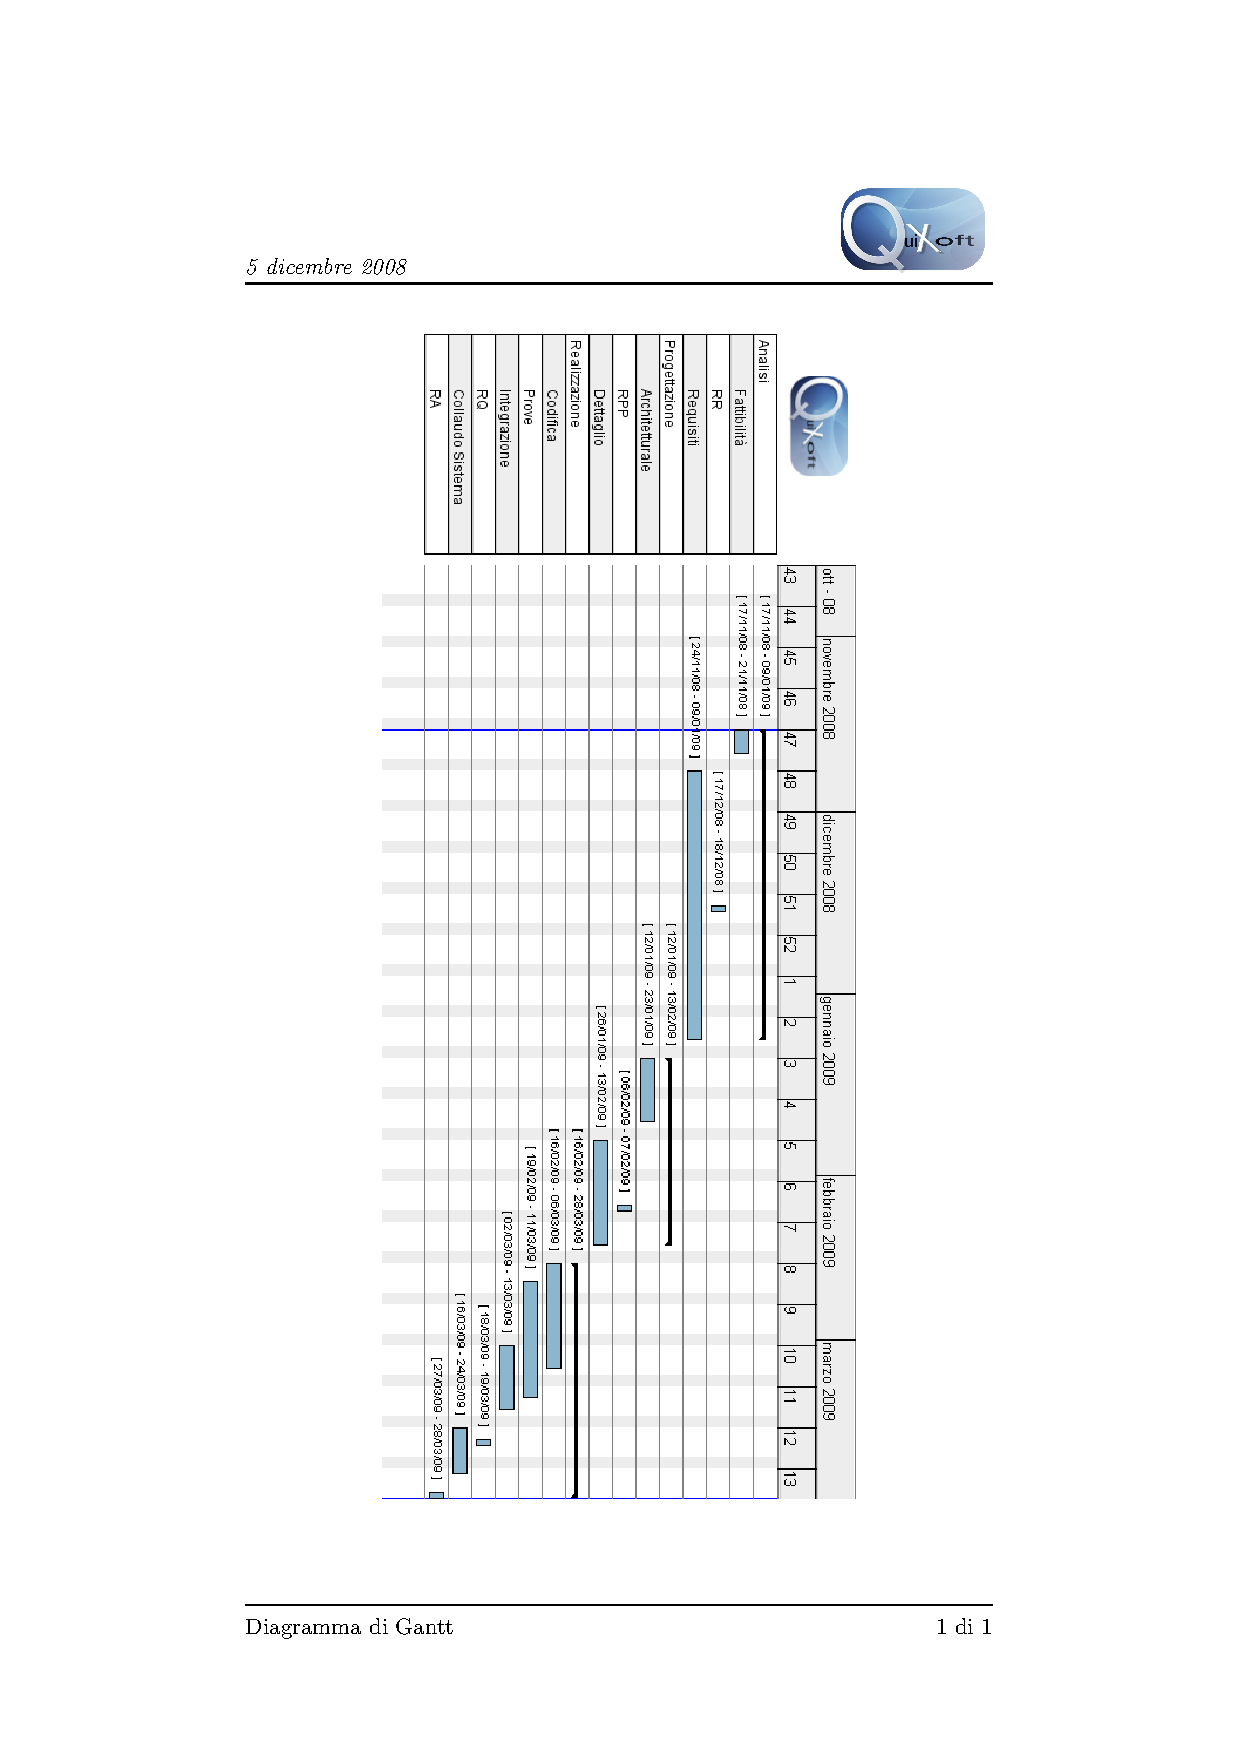
\includegraphics[scale=0.5]{gantt.png} \\

\subsection{Ore stimate nel progetto per ruolo}
La tabella sottostante mostra la suddivisione delle ore di ogni ruolo per ogni fase.\\

\begin{tabular}{|c|c|c|c|c|c|}
\hline
 & Analisi & Progettazione & Codifica & Ver.\&Val. & Totale \\ \hline
Responsabile & 22 & 14 & 14,5 & 12 & 62,5 \\ \hline
Amministratore & 19 & 20 & 26,5 & 17 & 82,5 \\ \hline
Analista & 120 & 0 & 0 & 0 & 120 \\ \hline
Progettista & 0 & 130 & 0 & 0 & 130 \\ \hline
Programmatore & 0 & 0 & 100 & 10 & 110 \\ \hline
Verificatore & 10 & 20 & 20 & 70 & 120 \\ \hline
\end{tabular}
\\

\subsection{Impegno individuale per ogni ruolo}
La tabella sottostante rappresenta le ore di ogni componente del team in relazione al ruolo ricoperto.\\

\begin{tabular}{|c|c|c|c|c|c|c|c|}
\hline
 & Barbiero & Beggiato & Freo & Grosselle & Scarpa & Scortecagna & Totale \\ \hline
Responsabile & 11 & 11 & 11 & 9,5 & 9 & 11 & 62,5 \\ \hline
Amministratore & 13,5 & 13,5 & 14,5 & 14 & 14 & 13 & 82,5 \\ \hline
Analista & 20 & 20 & 20 & 20 & 20 & 20 & 120 \\ \hline
Progettista & 21,5 & 22 & 21 & 22 & 21,5 & 22 & 130 \\ \hline
Programmatore & 19 & 18 & 18,5 & 18 & 18,5 & 18 & 110 \\ \hline
Verificatore & 20 & 20 & 20 & 20 & 20 & 20 & 120 \\ \hline
\end{tabular}

\section{Analisi dei rischi}
\subsection{Assenza componente per medio/lungo periodo}
Ogni componente ha sempre un determinato ruolo in tutte le fasi del progetto.
Se un componente risultasse indisponibile per un lasso di tempo piu' o meno lungo causerebbe un rallentamento del progetto se non addirittura uno stallo.
E' compito dell'amministratore riassegnare il determinato ruolo ad uno o piu' componenti del team e modificare il piano di progetto cercando di mantenere inalterati i costi e la data di fine progetto.
\subsection{Mancanza di conoscenze tecniche}
Si utilizzeranno strumenti e tecnologie che per alcuni utenti risulteranno nuove.
L'amministratore mettera' a disposizione guide e manuali per poter formare il team. Lo studio e' personale e non e' previsto nel piano di progetto. Tuttavia se dovesse essere necessario verra' fatta una riunione che delineara' i concetti di massima dello strumento o tecnologia.   
\subsection{Calendario delle attivita' inneficiente}
Le attivita', viste la scarsa esperienza, sono state pianificate basandosi su precedenti calendari di altri gruppi.
E' compito dell'amministratore correggere eventuali errori di pianificazione, cercando di mantenere inalterati i costi e la data di fine progetto.
\subsection{Analisi dei requisiti inefficiente}
Nella prima fase avviene lo studio approfondito dei requisiti. Finita questa fase, inizia quella di progettazione. Data la scarsa esperienza del team QuiXoft il rischio di variazione dei requisiti, dopo il loro studio esiste. Tuttavia si cerca di renderlo il piu' basso possibile ruotando il ruolo di analista e rendendo la ricerca dei requisiti il piu' completa ed efficiente possibile.
\subsection{Gestione della qualita' inadeguata}
L'accertamento della qualita' del processo e del prodotto e' garantita dalla presenza del ruolo del Verificatore per tutto il periodo di concezione e sviluppo del progetto. Se le ore necessarie al verificatore in una determinata fase dovessero essere troppo poche, verra' immediatamente avvisato l'amministratore che modifichera' il piano di progetto. 

\section{Conto economico preventivo}
\subsection{Costi stimati nel progetto per ruolo}
Dalla precedente pianificazione si può redigere la seguente tabella:\\

\begin{tabular}{|c|c|c|c|c|c|}
\hline
 & Analisi & Progettazione & Codifica & Verifica\&Valid. & Totale \\ \hline
Responsabile & 660 & 420 & 435 & 360 & 1875 \\ \hline
Amministratore & 380 & 400 & 530 & 340 & 1650 \\ \hline
Analista & 3000 & 0 & 0 & 0 & 3000 \\ \hline
Progettista & 0 & 2860 & 0 & 0 & 2860 \\ \hline
Programmatore & 0 & 0 & 1600 & 160 & 1760 \\ \hline
Verificatore & 160 & 320 & 320 & 1120 & 1920 \\ \hline
Totale & 4200 & 4000 & 3045 & 1820 & 13065 \\ \hline
\end{tabular}

\subsection{Costi stimati nel progetto per risorsa}
La tabella sottostante rappresenta i costi di ogni componente del team in relazione al ruolo ricoperto:\\

\begin{tabular}{|c|c|c|c|c|c|c|}
\hline
\multicolumn{1}{|l|}{} & \multicolumn{1}{l|}{        Barbiero} & \multicolumn{1}{l|}{          Beggiato} & \multicolumn{1}{l|}{              Freo} & \multicolumn{1}{l|}{               Grosselle} & \multicolumn{1}{l|}{          Scarpa} & \multicolumn{1}{l|}{  Scortecagna} \\ \hline
Responsabile & 330 & 330 & 330 & 285 & 270 & 330 \\ \hline
Amministratore & 270 & 270 & 290 & 280 & 280 & 260 \\ \hline
Analista & 500 & 500 & 500 & 500 & 500 & 500 \\ \hline
Progettista & 473 & 484 & 462 & 484 & 473 & 484 \\ \hline
Programmatore & 304 & 288 & 296 & 288 & 296 & 288 \\ \hline
Verificatore & 320 & 320 & 320 & 320 & 320 & 320 \\ \hline
Totale & 2197 & 2192 & 2198 & 2157 & 2139 & 2182 \\ \hline
\end{tabular}
\modifiche
\end{document}
